\documentclass[conference]{IEEEtran}
\IEEEoverridecommandlockouts
% The preceding line is only needed to identify funding in the first footnote. If that is unneeded, please comment it out.
%\usepackage{cite}
\usepackage{amsmath,amssymb,amsfonts}
\usepackage{algorithmic}
\usepackage{graphicx}
\usepackage{textcomp}
\usepackage{xcolor}
\def\BibTeX{{\rm B\kern-.05em{\sc i\kern-.025em b}\kern-.08em
    T\kern-.1667em\lower.7ex\hbox{E}\kern-.125emX}}

\usepackage{hyperref}
\usepackage{biblatex} 
\addbibresource{references.bib}

% To get bulletpoints inside a table cell
\usepackage{array}

% All images go in folder below
\graphicspath{{./pix/}} % put all your figures here.

\begin{document}

\title{Recognizing Activities of Daily Living Using Audio and IMU Data from Commodity Smartwatches
}

\author{
\IEEEauthorblockN{Yvette Espinoza}
\IEEEauthorblockA{\textit{Department of ECE} \\
\textit{Purdue University}\\
Los Angeles, CA \\
yespinoz@purdue.edu}

\and
\IEEEauthorblockN{Cameron Johnson}
\IEEEauthorblockA{\textit{Department of ECE} \\
\textit{Purdue University}\\
Asheville, NC \\
john3096@purdue.edu}

\and
\IEEEauthorblockN{Jahangir Mollah}
\IEEEauthorblockA{\textit{Department of ECE} \\
\textit{Purdue University}\\
Seattle, WA \\
jmollah@purdue.edu}
}

\maketitle

\begin{abstract}
Human activity recognition is applicable to healthcare, but there are limitations on devices that can be used.
The popularity of smart devices allow for comfort while also providing the data necessary to expand enable activity recognition.
In this project, smartwatches will be used to recognize activities of daily living.
\end{abstract}

%\begin{IEEEkeywords}
%component, formatting, style, styling, insert
%\end{IEEEkeywords}

\section{Introduction}

Early research in activity detection aimed at finding differences in signal characteristics of the collected accelerometer data, and determining the ideal sensor placement. 
In \cite{2011_Sensor_Positioning}, activities were grouped together into four categories by levels of physical activity, and sensors were placed throughout the body to determine the best location for each of the categories.
Their results found each category performed best with a different sensor location. A sensor placed on the waist was best at detecting low level activities like eating, while a sensor on the chest or wrist was best at medium level activities like housework.

While different sensor placement based on an activity would be ideal for performance, it would not be practical for widespread use.
An accelerometer by itself is not enough to determine an activity. More context is needed and different sensors on the body are an inconvenience for users. 
Human activity recognition is widely used in healthcare applications, with the elderly being a large part of the user demographics \cite{2018_Robust_Activity}, to suit their needs the data collection would require an unobtrusive setup.
To address the inconvenience of full body sensors and the need for context, \cite{2012_WristSense} used a wrist-worn device equipped with an accelerometer and camera to recognize daily activities. 
The camera provided context for the activities, and the accelerometer provided characteristics of the body movement associated with different activities, both of which were used to train a model to predict the activity.

The advancement in smart devices, like smartwatches and conversational assistants, allow for more sensors in a user friendly device.
Conversational assistants, like a Google Home, and smartwatches are used to train a model to recognize activities of daily living \cite{2021_Ok_Google} \cite{2022_Leveraging_sound}.

%\subsection{Machine Learning Algorithms}
% TODO - talk about the machine learning advances --> smart devies allow for more data collection, which allow for better ML models and classifiers %


\subsection{Motivation}
Audio monitoring can also be used to detect hazardous situations such as loud noises, falls, or emergencies. By integrating audio analysis into a smartwatch, users can be alerted to potential dangers in real-time, providing an added layer of safety.

Human activity recognition has potential applications that can be leveraged in healthcare, dietary monitoring, and weight management

We propose a research project, recognizing activities of daily living using the IMU and audio data from a commodity smartwatch. 
We will be following existing research performed in \cite{2022_Leveraging_sound}. 

\section{Methodology}
Our process will involve conducting experiments wearing a smartwatch and performing a variety of basic activities such as writing, brushing teeth, and washing hands. We will record IMU data and audio data using the mic on the watch as input to a deep learning model which fuses the inertial data and acoustic data to determine the activity being performed, shown in Figure \ref{fig: Architecture_of_Inertial_and_Acoustic_Models}. Recognizing activities of daily living using inertial data has been the focus of a number of studies in the recent past, but fewer studies have included acoustic data in the model. We believe using both types will result in more accurate recognition. Some activities such as writing are more easily captured using inertial data while other activities such as cutting paper are more captured using acoustic data.  Smart watches prove especially practical for recording both types of data because the mic is at close proximity to the hand which is often close to the activity being performed and the IMU records useful motion on the wrist as opposed to a smartphone in the pocket or strapped to the chest.

\begin{figure}[h]
    \centering
    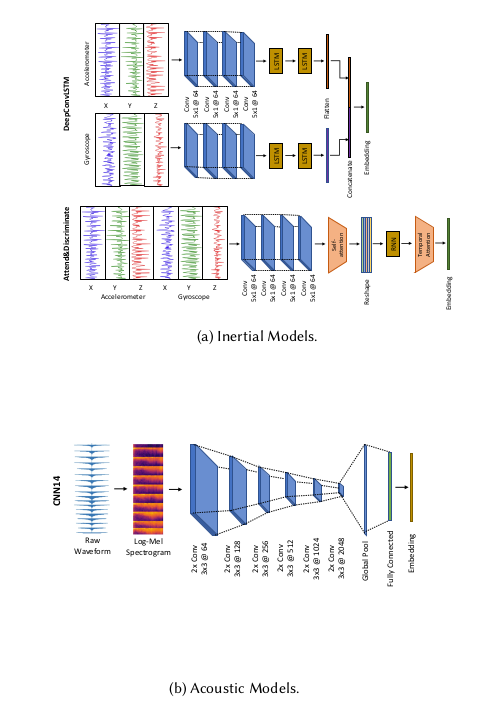
\includegraphics[scale=0.50]{Architecture_of_Inertial_and_Acoustic_Models}
    \caption{Architecture of Inertial and Acoustic Models, provided by \cite{2022_Leveraging_sound}}
    \label{fig: Architecture_of_Inertial_and_Acoustic_Models}
\end{figure}

\subsection{Hardware Setup}
The authors of \cite{2022_Leveraging_sound} used the same watch for all of their experiments. They used a Fossil Gen 4, Android Wear OS 2.21, Custom application collects data synchronously and stores locally on watch. Max inertial sensor samples at rate 50 Hz, acoustic sampled at 22.05 KHz. We will be using different watch manufacturers in our experiment to ensure generic compatibility.

\subsection{Original Experimental Setup and Results}
The paper that we follow conducted two generally different experiments. In the first experiment, an individual performs a series of activities for 30 seconds wearing a Fossil smartwatch which records inertial and acoustic data. There is a clear distinction between each activity and the watches are programmed to listen at frequent intervals. The authors implemented a variety of machine learning models to recognize the activity in this experiment with an accuracy of 94.3. The second experiment implements a less controlled, more realistic setting.
One limitation of this paper was that their not controlled experiment had poor results due to noise and mislabeling of activities due to the setup.
Since their experiment was not controlled, not all the activities they were interested in were performed, in some cases activities overlapped, and combined with a limited sample size resulted in misclassifications.

For our project we plan to expand our sample size and have a more controlled environment.
We intend to focus on recognizing an activity on command, in a more controlled environment where we set rules to prevent the noise and mislabeling seen in the original paper.

% TODO: [Describe] Accuracy of 55.8.

\subsection{Schedule}
The project was divided into four phases.
More details on due dates and deliverables for each phase are provided in Table \ref{tab: Schedule}.

\begin{table}[htbp]
	\caption{Schedule}
	\begin{center}
		\begin{tabular}{| m{1.2cm} | m{4cm} | m{1.2cm} |}
			\hline
			\textbf{Phase} & \textbf{Activities} & \textbf{Due Date} \\
			\hline
			Planning & 
			\begin{itemize}
				\item Identify existing research data
				\item Identify available hardware
				\item Plan for how to capture and store data
				\item Identify how to process data
				\item Identify machine learning classification models
			\end{itemize} &
			March 18 \\
			\hline
			
			Data Collection & 
			\begin{itemize}
				\item Capture and process raw data
				\item Capture audio data at all times
				\item Review existing research data
				\item Get volunteers for experiments
			\end{itemize} & 
			April 1 \\
			\hline
			
			Analysis & 
			\begin{itemize}
				\item Fuse data collected from different sources
				\item Label data collected
				\item Run the classification models
				\item Analyze results
			\end{itemize} & 
			April 15 \\
			\hline
			
			Finalize Report & 
			\begin{itemize}
				\item Write up final report
				\item Create presentation
			\end{itemize} & 
			April 22 \\
			\hline
		\end{tabular}
		\label{tab: Schedule}
	\end{center}
\end{table}

\section*{Acknowledgment}

Paper we are implementing \cite{2022_Leveraging_sound}.

\nocite{*}
\printbibliography

\end{document}
